\documentclass[14pt, oneside]{altsu-report}

\worktype{Создание программы}
\title{Курсовая работа (2 курс)}
\author{А.\,П.~Скопич}
\groupnumber{2.205-1}
\GradebookNumber{1337}
\supervisor{И.\,А.~Шмаков}
\supervisordegree{ст. преп. каф. ВТиЭ}
\ministry{Министерство науки и высшего образования}
\country{Российской Федерации}
\fulluniversityname{ФГБОУ ВО Алтайский государственный университет}
\institute{Институт цифровых технологий, электроники и физики}
\department{Кафедра вычислительной техники и электроники}
\departmentchief{В.\,В.~Пашнев}
\departmentchiefdegree{к.ф.-м.н., доцент}
\shortdepartment{ВТиЭ}
\abstractRU{Большой текст на русском! Пока счётчик работает не правильно! Поправьте количество рисунков и таблиц в cls-файле.}
\abstractEN{Большой текст на английском!}
\keysRU{Python, tkinter, программа, стуктура, код}
\keysEN{computer simulation, distributed version control}

\date{\the\year}

% Подключение файлов с библиотекой.
\addbibresource{graduate-students.bib}

% Пакет для отладки отступов.
%\usepackage{showframe}

\begin{document}
\maketitle

\setcounter{page}{2}
\makeabstract
\tableofcontents

\chapter*{Введение}
\phantomsection\addcontentsline{toc}{chapter}{ВВЕДЕНИЕ}

\textbf{Актуальность: }
С того момента, когда игры были только средством развлечения прошло не так много времени. Быстрый рост игровой индустрии привели к крупным изменениям в жизни людей. Сейчас разработчики создают игры, способные научить детей считать, или симуляторы, помогающие будущим профессионалам ознакомиться с их деятельностью практически напрямую. Но, не смотря на такой широкий выбор, игры до сих пор сохраняют ту функцию, для которой они были изначально созданы: развлечение, расслабление и "коротание времени".

\textbf{Цель: }
Разработать программу - классическую игру "Танчики" на языке программирования Python с обязательным использованием библиотеки tkinter.

\textbf{Задачи:}
\begin{enumerate}
\item Теоритическая часть.
\begin{enumerate}
    \item Изучить функционал библиотеки tkinter.
    \item Рассмотреть и изучить примеры подобных игр, написанных в среде программирования Python.
    \item Описать вид и функциональные возможности игры.
    \item Разработать блок-схему программы;
\end{enumerate}
\item Практическая часть.
\begin{enumerate}
    \item Написать код программы (основного функционала игры);
    \item Провести тестирование программы;
    \item Дополнить функционал программы;
\end{enumerate}
\item Написать отчёт по выполненной работе.
\end{enumerate}

% Подключение первой главы (теория):
\chapter{\label{ch:ch01}ГЛАВА 1: ТЕОРИТИЧЕСКАЯ ЧАСТЬ} % Нужно сделать главу в содержании заглавными буквами

\section{\label{sec:ch01/sec01}Раздел 1: Изучение языка Python и библиотеки tkinter}

Мне потребовалось освежить и немного расширить свои знания по языку Python. Для этого я воспользовался книгами по Питону "Python. Подробный справочник"~\cite{book_Python} и "УЧИМ PYTHON, ДЕЛАЯ КРУТЫЕ ИГРЫ"~\cite{book_Python_2}.

Затем я рассмотрел основы написания программ с использованием библиотеки tkinter ~\cite{Python-tkinter},
ещё мне помог сайт pythonpip.ru про Python и tkinter ~\cite{Python-tkinter_2} и сайт-курс по tkinter ~\cite{Course-tkinter}.

\section{\label{sec:ch01/sec02}Раздел 2: Изучение кода программ других разработчиков}

Чтобы разобраться, как пишутся именно игры на Python, я должен был рассмотреть конкретные примеры. Сайт github предоставил прекрасную возможность изучить простенькие игры.

%При помощи этой программы уже можно заметить основную структуру однофайловой программы, которую я позаимствую для написания своей программы.

\section{\label{sec:ch01/sec03}Раздел 3: Задумка и основные функции}

Моей программой должна стать игра "Танчики". Это должно быть, в первую очередь, игровое поле, сосотоящее из блоков (кирпичных и железных стен). В ней игроку предстоит перемещаться по игровом полю и побеждать вражеские танки, за уничтожение танка начисляются очки, которые формируют счет игрока. Игра продолжается до тех пор, пока танк игрока не будет уничтожен.

Само игровое поле будет иметь возможность редактировать размер, состав и расположение объектов на ней, при это будет менять и размер окна программы.

\section{\label{sec:ch01/sec04}Раздел 4: Структура программы}

В данном разделе будут описаны все составляющие игры.

\subsection{\label{sec:ch01/sec04/sub01}Игровое меню}

Игровое меню - это то, с чего начинается программа сразу после запуска. Это будет окно размером 800*600 пикселей, содержащий на себе название игры и список кнопок, по которым будет происходить переход.

\subsection{\label{sec:ch01/sec04/sub02}Настройки}

Один из переходов в программе, к которой можно перейти из главного меню. Он будет содержать такие опции, как возможность создать свое собственное поле с желаемыми размерами и разместить на них игровые объекты (кирпичные, железные блоки) либо выбрать поле по умолчанию.

\subsection{\label{sec:ch01/sec04/sub03}Окно "О разработчике"}

Это окно будет выводиться по нажатии кнопки "Разработчик" в главном меню. Оно будет содержать информацию Фамилии, Имени и группы студента, разрвботавшего данную программу.

\subsection{\label{sec:ch01/sec04/sub04}Игровое поле}

Это онсновной цикл в программе, в котором на холсте (окне игры) будут размещаться игровые объекты, происходить взаимодействия между объектами, игроку будет предоставлено управление с клавиатуры.

Размер окна в этом разделе будет варьироваться от количества блоков игрового поля в ширину и высоту (количество блоков * размер блока) (но не равны нулю, само собой).
% Подключение второй главы (практическая часть):
\chapter{\label{ch:ch02}ПРАКТИЧЕСКАЯ ЧАСТЬ}

% Подключение третий главы (практическая часть с тестированием:
\chapter{\label{ch:ch03}ПРОДОЛЖЕНИЕ ПРАКТИЧЕСКОЙ ЧАСТИ}

Пример ссылок:
\begin{enumerate}
\item на главу~\ref{ch:ch01};
\item на раздел~\ref{sec:ch01/sec01} главы~\ref{ch:ch01};
\item на раздел~\ref{sec:ch02/sec01} главы~\ref{ch:ch02};
\item на приложение на странице~\pageref{appendix1};
\item на код на странице~\pageref{code:pi-example}.
\end{enumerate}

\section{\label{sec:ch03/sec01}Раздел 1}

\subsection{\label{subsec:ch03/sec01/sub01}Подраздел 1}

\subsection{\label{subsec:ch03/sec01/sub02}Подраздел 2}

\section{\label{sec:ch03/sec02}Раздел 2}

\subsection{\label{subsec:ch03/sec02/sub01}Подраздел 1}

\subsection{\label{subsec:ch03/sec02/sub02}Подраздел 2}

Пример ссылки на рисунок в документе~\ref{fig:example05}.
\begin{figure}[h]
    \centering
    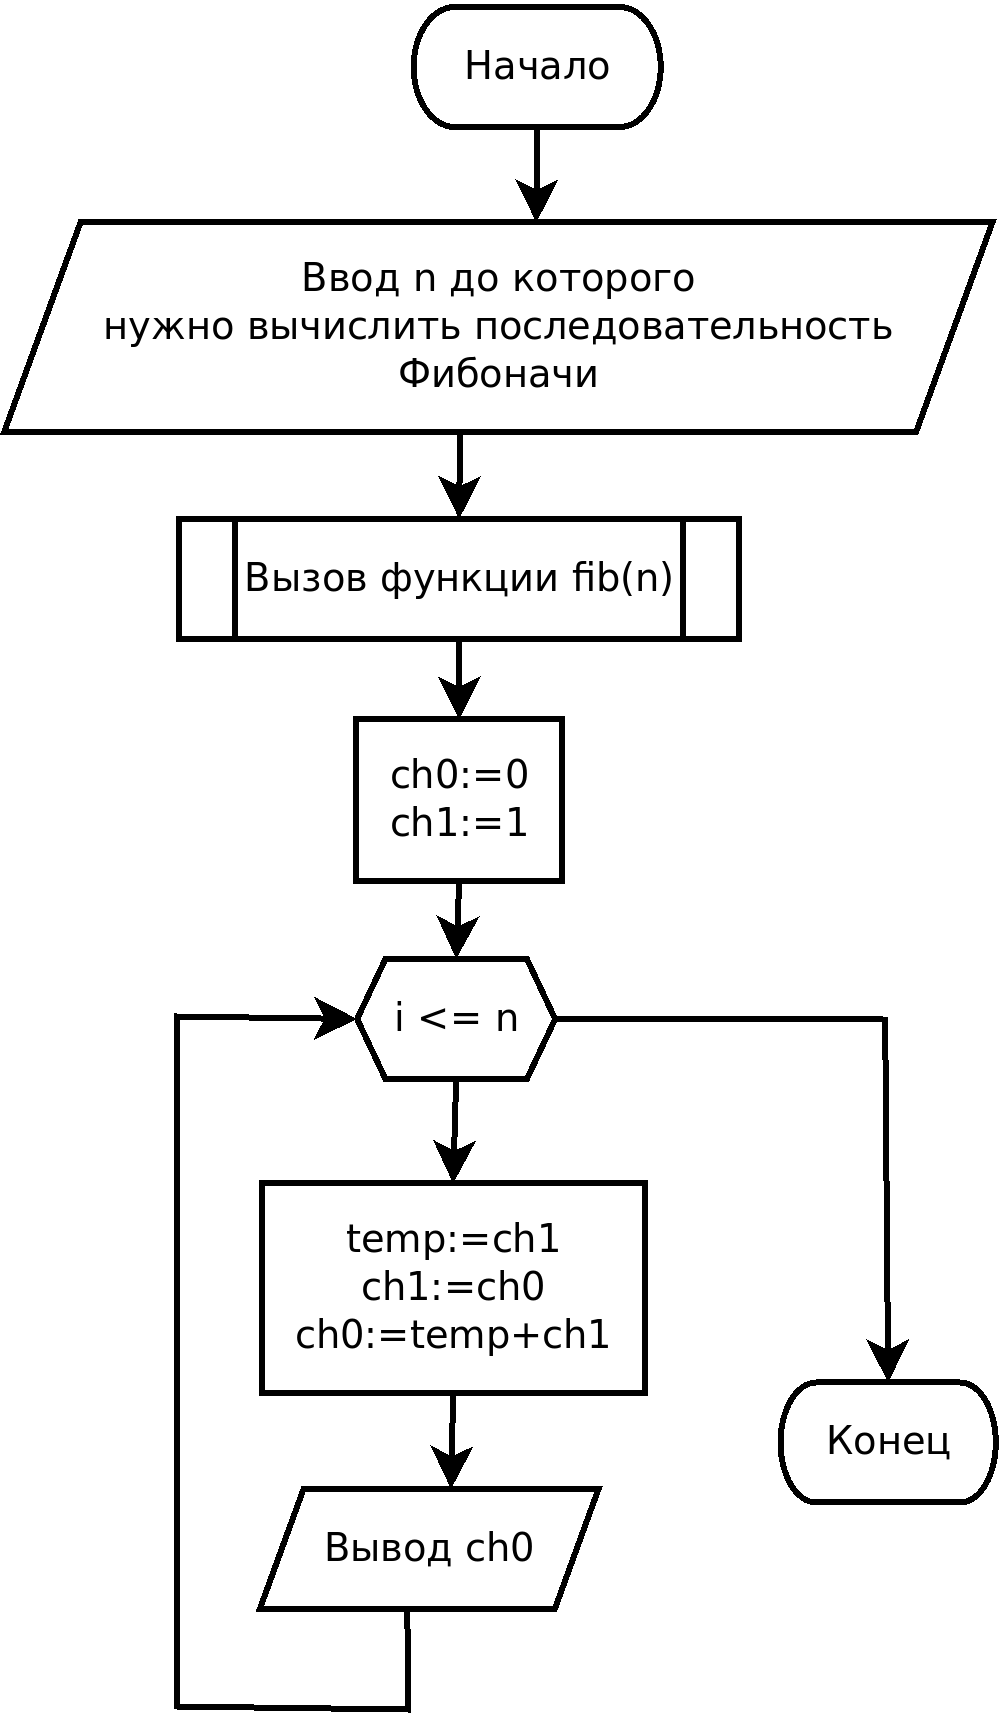
\includegraphics[width=0.5\textwidth]{./images/fibonacci.png}
    \caption{\centering\label{fig:example05}Пример рисунка в формате PNG.}
\end{figure}

Пример ссылки на рисунок в документе~\ref{fig:example06}.
\begin{figure}[h]
    \centering
    \includesvg[width=0.5\textwidth]{./images/fibonacci.svg}
    \caption{\centering\label{fig:example06}Пример рисунка в формате SVG.}
\end{figure}

Пример ссылки на таблицу в документе~\ref{tab:example05}.
\begin{table}[H]
\caption{\centering\label{tab:example05}Системные требования}
\begin{tabular}{|p{3 cm}|p{3 cm}|p{3 cm}|p{5 cm}|}
\hline
Минимальные требования & 1 & 2 & 3 \\ \hline
Версия операционной системы & 1 & 2 & 3 \\ \hline
Процессор & 1 & 2 & 3 \\ \hline
Графический API & 1 & 2 & 3 \\ \hline
\end{tabular}
\end{table}

Пример ссылки на таблицу в документе~\ref{tab:example06}.
\begin{table}[H]
\caption{\centering\label{tab:example06}Системные требования}
\begin{tabular}{|p{3 cm}|p{3 cm}|p{3 cm}|p{5 cm}|}
\hline
Минимальные требования & 1 & 2 & 3 \\ \hline
Версия операционной системы & 1 & 2 & 3 \\ \hline
Процессор & 1 & 2 & 3 \\ \hline
Графический API & 1 & 2 & 3 \\ \hline
\end{tabular}
\end{table}

Пример использования minted для оформления кода и ссылка на этот код~\ref{code:example05}.
\begin{code}
\captionof{listing}{\centering\label{code:example05}Вычисление последовательности Фибоначчи}
\vspace{-\baselineskip}\begin{minted}{C}
#include <stdio.h>
#include <omp.h>
#define N 100

int main(int argc, char *argv[]) {
  double a[N], b[N], c[N];
  int i;
  omp_set_dynamic(0); // запретить библиотеке openmp менять число потоков во время исполнения
  omp_set_num_threads(10); // установить число потоков в 10
  // инициализируем массивы
  for (i = 0; i < N; i++) {
      a[i] = i * 1.0;
      b[i] = i * 2.0;
  }
  // вычисляем сумму массивов
#pragma omp parallel for shared(a, b, c) private(i)
   for (i = 0; i < N; i++)
     c[i] = a[i] + b[i];

  printf ("%f\n", c[10]);
  return 0;
}
\end{minted}
\end{code}

Пример использования minted для оформления кода и ссылка на этот код~\ref{code:example06}.
\begin{code}
\captionof{listing}{\centering\label{code:example06}Сложение двух массивов параллельно десятью потоками (пример из https://ru.wikipedia.org/wiki/OpenMP)}
\vspace{-\baselineskip}\begin{minted}{C}
#include <stdio.h>
#include <omp.h>
#define N 100

int main(int argc, char *argv[]) {
  double a[N], b[N], c[N];
  int i;
  omp_set_dynamic(0); // запретить библиотеке openmp менять число потоков во время исполнения
  omp_set_num_threads(10); // установить число потоков в 10
  // инициализируем массивы
  for (i = 0; i < N; i++) {
      a[i] = i * 1.0;
      b[i] = i * 2.0;
  }
  // вычисляем сумму массивов
#pragma omp parallel for shared(a, b, c) private(i)
   for (i = 0; i < N; i++)
     c[i] = a[i] + b[i];

  printf ("%f\n", c[10]);
  return 0;
}
\end{minted}
\end{code}


\chapter*{Заключение}
\phantomsection\addcontentsline{toc}{chapter}{ЗАКЛЮЧЕНИЕ}

Были изучены язык программирования Python и некоторые его библиотеки, в особенности tkinter, структура написания программ. Рассмотрены примеры похожих простых программ - игр от других разработчиков. Написана работоспособная программа "Танчики".

\newpage
\phantomsection\addcontentsline{toc}{chapter}{СПИСОК ИСПОЛЬЗОВАННОЙ ЛИТЕРАТУРЫ}
\printbibliography[title={Список использованной литературы}]

\appendix
\newpage
\chapter*{\raggedleft\label{appendix1}Приложение}
\phantomsection\addcontentsline{toc}{chapter}{ПРИЛОЖЕНИЕ}

\end{document}

